\section{General description}

The GeoPAT consists of twelve modules (Fig. \ref{FIG:GPAT}).
Five modules are designed for extracting pattern signatures from an original data grid, four modules for actual geoprocessing of the patterns, and three utility modules.

\begin{figure}[H]
 	\centering
	\makebox[\textwidth][c]{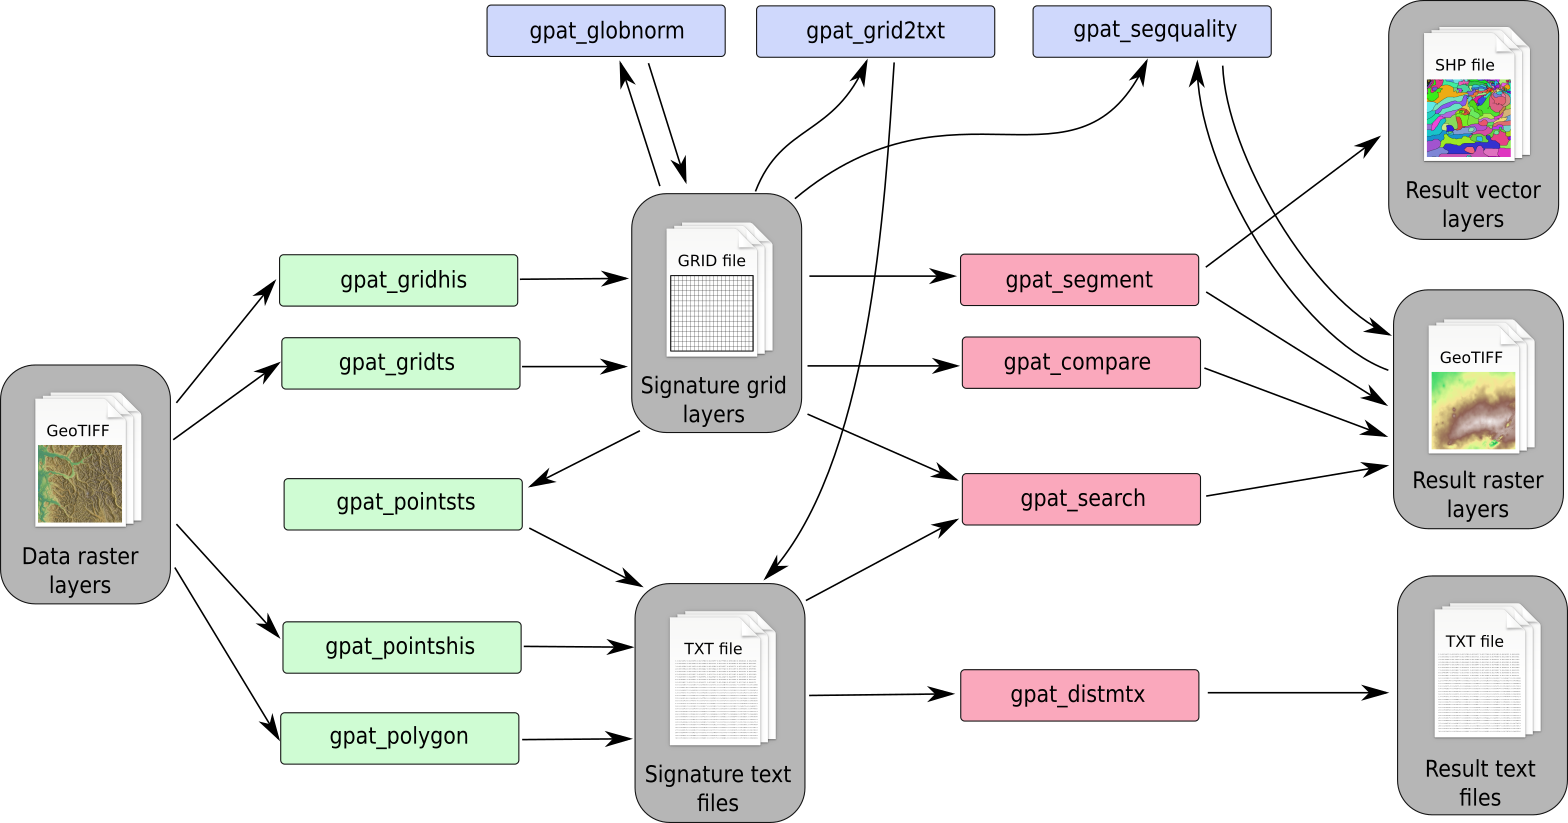
\includegraphics[width=1.1\textwidth]{GPAT.png}}
	\caption{Outline of the GeoPAT 2 architecture}
	\label{FIG:GPAT} 
\end{figure}

The role of signature extraction modules ({\tt gpat\_gridhis}, {\tt gpat\_gridts}, {\tt gpat\_pointshis}, {\tt gpat\_pointsts}, {\tt gpat\_polygon}) is to calculate pattern signatures for scenes defined:

\begin{itemize}
  \item \texttt{gpat\_gridhis} - by a neighborhood of each cell in a grid (spatial pattern)
  \item \texttt{gpat\_gridts} - by a neighborhood of each cell in a grid (spatiotemporal pattern)
  \item \texttt{gpat\_pointshis} - in the neighborhoods of selected points (spatial pattern)
  \item \texttt{gpat\_pointsts} - in the neighborhoods of selected points (spatiotemporal pattern)
  \item \texttt{gpat\_polygon} - over irregular polygons
\end{itemize}

The role of geoprocessing modules ({\tt gpat\_search}, {\tt gpat\_compare}, {\tt gpat\_segment}, {\tt gpat\_distmtx}) is to perform:

\begin{itemize}
  \item \texttt{gpat\_search} - searching
  \item \texttt{gpat\_compare} - comparision
  \item \texttt{gpat\_segment} - segmentation (based on pattern data generated by the signature extraction modules)
  \item \texttt{gpat\_distmtx} - clustering
\end{itemize}

The role of utility modules ({\tt gpat\_grid2txt}, {\tt gpat\_globnorm}, {\tt gpat\_segquality}) is to:

\begin{itemize}
  \item \texttt{gpat\_grid2txt} - convert grid of signatures (grid-of-scenes) from a binary to text
  \item \texttt{gpat\_globnorm} - normalization of grid of signatures (grid-of-scenes) values
  \item \texttt{gpat\_segquality} - calculate the quality metrics (inhomogeneity and isolation) of a segmentation
\end{itemize}

\section{GeoPAT Modules}

\subsection{Signature building}

\subsubsection{gpat\_gridhis}
Creates a binary grid of signatures from a categorical raster map(s).
\\\\
Usage:

\begin{minipage}{\linewidth}
\begin{lstlisting}
gpat_gridhis [-lh] -i <file_name> -o <file_name> [-s <signature_name>] [--level=<n>] [-z <n>] [-f <n>] [-n <normalization_name>] [-t <n>]

-i, --input=<file_name>    name of input file (GeoTIFF)
-o, --output=<file_name>   name of output file (GRID)
-s, --signature=<name>     motifel's signature (use -l to list all signatures, default: 'cooc')
--level=<n>                full decomposition level (default: auto)
-z, --size=<n>             motifel size in cells (default: 150)
-f, --shift=<n>            shift of motifels (default: 100)
-n, --normalization=<name> signature normalization method (use -l to list all methods, default: 'pdf')
-l                         list all signatures and normalization methods
-t <n>                     number of threads (default: 1)
-h, --help                 print this help and exit
\end{lstlisting}
\end{minipage}

{\bf Options:}

\newoption{input}

Defines a categorical raster layer(s) which will be used as a source for extracting pattern signature.
Layers must be a categorical one. 
For the Cartesian product method ('prod') there can be more than one input map.
In order to provide more than one input map, type multiple input options ("-i map1.tif -i map2.tif" or "--input=map1.tif --input=map2.tif").
Other methods use a one map only (the first one provided). 

\newoption{output}

Output consists of two files: one of them is a dataset containing a grid of signatures in binary form, the other one is a header text file (the .hdr extension) containing a grid topology and information about the input data parameters.
Modifying the header is strongly discouraged as it may cause some calculations to fail. 
Structure of the header is as follows:\\

\begin{itemize}
	\item dim -- number of dimensions of each signature
	\item dims -- size of each dimension
	\item type -- type of data stored in the grid (integer, float, etc.)
	\item at0 -- top left x
	\item at1 -- w-e grid resolution
	\item at2 -- rotation (0 if grid is north-up)
	\item at3 -- top left y
	\item at4 -- rotation (0 if grid is north-up)
	\item at5 -- n-s grid resolution
	\item rows -- number of rows in the grid
	\item cols -- number of cols in the grid
	\item proj -- projection in wkt style
	\item desc -- command used to create the grid
\end{itemize}

\newoption{size}

Size of a motifel (local calculation window) expressed in the number of pixels. 
It defines the extent of a local pattern.
It is the length of the side of square-shaped block of pixels (motifel).
It must be at least 10 and cannot exceed the input map size.

\newoption{shift}

Parameter defines the shift between adjacent scenes along the grid in n-s and w-e directions. 
It describes the density of the output gird and defines a new topology of the grid.
Formula original\_resolution $\times$ shift = new\_resolution explains how resolution of the original map will be reduced. 
If shift is set to the same value as 'size', the input map will be simply divided into a grid of non-overlapping motifels. 
Setting shift to a value smaller than 'size' parameter will result in grid of overlapping motifels. 
Shift cannot be larger than 'size', and cannot be smaller than 5.

\newoption{signature}

Defines method of calculating signatures of motifels. GeoPAT offers the following methods: 
\begin{itemize}
	\item prod -- Cartesian product of input category lists
	\item cooc -- Spatial coocurrence of categories
	\item fdec -- Full decomposition
	\item lind -- Landscape indices vector
	\item linds -- Selected landscape indices vector
	\item ent -- Shannon entropy
\end{itemize}
See Appendix \ref{signatures} for the details.

\newoption{level}

This option is used only if 'full decomposition' (fdec) is used.
It defines the highest level of decomposition. See Appendix \ref{signatures} for the details.

\newoption{normalization}

Specifies normalization method used on the local signatures. 
See Appendix \ref{normalization} for the details.
Normalization method used should depend on a selected signature method. 
For example, the default pdf normalization works well for the histogram-based signatures (pred, cooc, fdec), while normalization should be disabled (none) for the landscape indices signatures (lind, linds) and the Shannon entropy signature.

\newoption{threads (-t)}

The module is parallel, therefore use more than one processing thread can be used in order to speed up calculations. 
This option specifies how many threads will be used. 
The default is 1.
\\\\

{\bf Description:}

This module extracts a "grid-of-scenes" (grid of pattern signatures, grid of motifels).
The output is a grid of the same spatial extent as the input raster map, but with a different cell size.
Each cell in a new grid has only one attribute - the signature of its pattern. 
Pattern is calculated over a window centered on the cell and having a user-defined size.
Resolution of the output grid equals to the resolution of the input raster map multiplied by the shift parameter. 
A signature of pattern for each scene is stored as a numerical vector in a binary form.
The module outputs a header file (.hdr) containing a topology of a grid-of-scenes and a binary file containing signatures ordered by rows.

This module uses categorical raster data in GeoTIFF format as an input. 
It might be more than one map for the Cartesian product signature. 
Raster maps must be categorical and its size must be greater than the scene size specified by the user. 
Size defines the size of individual scene for which the histogram is calculated. 
Shift shows how scenes shift along the grid in n-s and w-e directions. 
Shift defines the resolution of the new grid.
If window size is bigger than shift (recommended), motifels will overlap.
If shift and size is equal, windows will not overlap. Shift cannot be greater than size. 

The output grid may be an input to one of the following GeoPAT modules: {\tt gpat\_search, gpat\_compare, gpat\_segment, gpat\_segquality, gpat\_grid2txt, and gpat\_globnorm}.

\subsubsection{gpat\_gridts}

\textbf{This feature is experimental.}
Creates a grid of time series signatures from raster maps.
\\\\
Usage:

\begin{minipage}{\linewidth}
\begin{lstlisting}
gpat_gridts [-nh] -i <file_name> [-i <file_name>]... -o <file_name> [-d <n>]

-i, --input=<file_name>  name of input file(s) (GeoTIFF)
-o, --output=<file_name> name of output file (GRID)
-d, --dimension=<n>      dimension of vector that describes time series element (default: 1)
-n, --normalize          normalize each vector coordinate to [0.0, 1.0] (default: no)
-h, --help               print this help and exit
\end{lstlisting}
\end{minipage}

\newoption{input}

Defines raster layers that will be used as a source for building time series grid.
Number of input layers has to be equal to the time series length times the size of time series element.
In order to provide input maps, type multiple input options ("-i map1.tif -i map2.tif" or "--input=map1.tif --input=map2.tif").
The order of the input layers is important. 
Following time series has length of six and each element contains three attributes:

\begingroup
\begin{equation} \label{eq:time_serie}
ts = \begin{bmatrix}
attr_{1,1}, & attr_{2,1}, &  attr_{3,1} \\ 
attr_{1,2}, & attr_{2,2}, &  attr_{3,2} \\ 
attr_{1,3}, & attr_{2,3}, &  attr_{3,3} \\ 
attr_{1,4}, & attr_{2,4}, &  attr_{3,4} \\
attr_{1,5}, & attr_{2,5}, &  attr_{3,5} \\
attr_{1,6}, & attr_{2,6}, &  attr_{3,6}
\end{bmatrix}
\end{equation}
\endgroup

For such time series input, GeoTiff (each GeoTiff contains one attribute) files should be in following order:
$attr_{1,1}$, $attr_{2,1}$, $attr_{3,1}$,
$attr_{1,2}$, $attr_{2,2}$, $attr_{3,2}$, 
 ... 
$attr_{1,5}$, $attr_{2,5}$, $attr_{3,5}$,
$attr_{1,6}$, $attr_{2,6}$, $attr_{3,6}$.

In this case a call of {\tt gpat\_gridts} should look like: \\

\begin{minipage}{\linewidth}
\begin{lstlisting}
gpat_gridts -i attr11.tif -i attr21.tif -i attr31.tif -i attr12.tif, ... -o new_grid
\end{lstlisting}
\end{minipage}

\newoption{output}

Output consists of two files: one of them is a dataset containing the grid of time series in the binary form, the other one is a header text file (the .hdr extension) containing the grid topology and the information about the input data parameters.
Modifying the header is strongly discouraged as it may cause some calculations to fail. 
Structure of the header is as follows:\\

\begin{itemize}
	\item dim -- number of dimensions (for time series it is 2)
	\item dims -- size of each dimension (two numbers: size of time series element, length of time series)
	\item type -- type of data stored in the grid (integer, float, etc.)
	\item at0 -- top left x
	\item at1 -- w-e grid resolution
	\item at2 -- rotation (0 if grid is north-up)
	\item at3 -- top left y
	\item at4 -- rotation (0 if grid is north-up)
	\item at5 -- n-s grid resolution
	\item rows -- number of rows in the grid
	\item cols -- number of cols in the grid
	\item proj -- projection in the wkt style
	\item desc -- command used to create the grid
\end{itemize}

\newoption{dimension}

The dimension of a time series element. 
This number describes length of vectors that builds a time series.

\newoption{normalize}

An option to normalize each attribute to $[0.0, 1.0]$ globally.\\

{\bf Description:}

This module creates a grid of time series (grid of time pattern signatures).
The output is a grid of the same spatial extent as the input raster map, with the same cell size.
Time series are stored as numerical vectors in the binary form.
The module outputs a header file (.hdr) containing a topology of the grid and a binary file containing the time series ordered by rows.

This module uses raster data in the GeoTIFF format as an input. 
Number of input files has to be equal to number of the time series element dimension.

The output grid may be an input to one of the following GeoPAT modules: {\tt gpat\_pointsts}, {\tt gpat\_search}, {\tt gpat\_compare}, {\tt gpat\_segment}, {\tt gpat\_segquality}, {\tt gpat\_grid2txt}, and {\tt gpat\_globnorm}.

\subsubsection{gpat\_pointshis}
Calculates numerical signatures of individual motifels within a raster map.
\\\\
Usage:

\begin{minipage}{\linewidth}
\begin{lstlisting}
gpat_pointshis [-lah] -i <file_name> -o <file_name> [-s <signature_name>] [--level=<n>] [-z <n>] [-n <normalization_name>] [-x <double>] [-y <double>] [-d <string>] [--xy_file=<file_name>]

-i, --input=<file_name>    name of input file (GeoTIFF)
-o, --output=<file_name>   name of output file (TXT)
-s, --signature=<name>     motifel's signature (use -l to list all signatures, default: 'cooc')
--level=<n>                full decomposition level (default: 0, auto)
-z, --size=<n>             motifel size in cells (default: 150)
-n, --normalization=<name> signature normalization method (use -l to list all methods, default: 'pdf')
-l                         list all signatures and normalization methods
-x <double>                x coord
-y <double>                y coord
-d, --description=<string> description of the location
--xy_file=<file_name>      name of file with coordinates (TXT)
-a, --append               append results to output file
-h, --help                 print this help and exit
\end{lstlisting}
\end{minipage}

{\bf Options:}

\newoption{input}

Defines categorical raster map(s) in the GeoTIFF format, which will be used as a source for extracting pattern signature.
For the Cartesian product method ('prod') there can be more than one input map. 
Other methods use one map only (the first one provided). 
In order to provide more than one input map, type multiple input options ("-i map1.tif -i map2.tif" or "--input=map1.tif --input=map2.tif").

\newoption{output}

Name of output text file containing signatures. 
In the output file, each line corresponds to a single motifel's signature. 
Each signature is preceded by its header.
A header always consists of: coordinates of the midpoint of motifel (scene), name, number of dimensions, and length of each dimension. 
Modifying the signature file is strongly discouraged as it may cause some calculations to fail.

\newoption{signature}

Defines method for calculating signatures of motifels.
GeoPAT offers the following methods: 
\begin{itemize}
	\item prod -- Cartesian product of input category lists
	\item cooc -- Spatial coocurrence of categories
	\item fdec -- Full decomposition
	\item lind -- Landscape indices vector
	\item linds -- Selected landscape indices vector
	\item ent -- Shannon entropy
\end{itemize}
See Appendix \ref{signatures} for details.

\newoption{level}

This option is used only when 'full decomposition' (fdec) is used.
It defines the highest level of decomposition.
See Appendix \ref{signatures} for the details.

\newoption{size}

Size of a motifel (scene) for which signature is calculated.
Scene is a square centered at the coordinate pair location, while its extent is defined by size. 

\newoption{normalization}

Specifies normalization method used on the local signatures. 
See Appendix \ref{normalization} for the details.
Normalization method used should depend on a selected signature method. 
For example, the default pdf normalization works well for the histogram-based signatures (pred, cooc, fdec), while normalization should be disabled (none) for the landscape indices signatures (lind, linds) and the Shannon entropy signature.

\newoption{x}

X coordinate of the midpoint of motifel for which signature will be calculated.

\newoption{y}

Y coordinate of the midpoint of motifel for which signature will be calculated.

\newoption{description}

Description of a motifel.
It can be a name of location, description of pattern, or anything else. 
If not provided, the default description is "location".

\newoption{xy\_file}

Name of a text file with list of coordinates. 
This option is useful for calculating signatures for multiple motifels in a single run. 

\newoption{append} (flag)

Append mode. 
Useful when using the coordinate pair mode and when scenes are processed one by one (see description below). 
If the append flag is used and the output file already exists, signatures will be appended at the end of file instead of overwriting it.
\\\\
{\bf Description:}

This module extracts signatures for a scene (motifel) or collection of scenes defined over square-shaped windows.
User provides coordinates of the center of each scene and the size of the scene. 
The module outputs a list of scene-labeled signatures.
As an input the module uses categorical raster map in the GeoTIFF format (or a few maps if user calculates the Cartesian product of multiple maps), coordinates of the center of each scene and size of scenes. 
The coordinates must be in the input map's coordinate system. 
There are two ways of defining the scenes:

Definition by coordinate pair: 
This is the simplest mode designed for a batch or interactive processing. 
In this mode, scene is defined by a pair of its midpoint's coordinates (the {\it x} and {\it y} options) and scene size parameter (the {\it size} option). 
Only one scene can be processed at once. 
The {\it xy\_file} option is not used in this mode.
If used with the append flag (-a), signatures can be calculated one by one and added to the same output file. 
Additionally, the {\it description} option lets user name a scene. 
This name will be stored in the output file.

Definition by text file:
In this mode, scene midpoint's coordinates are defined in a external text file in which each line contains X,Y coordinates using the following syntax: x\_coordinate,y\_coordinate.
The name of a file with coordinates is provided using the {\it xy\_file} option. 
Extent of a scene is defined by the {\it size} parameter. 
The {\it x, y} and {\it description} options are not used in this mode. 
Example of the content of coordinates file: 

\begin{minipage}{\linewidth}
\begin{lstlisting}
1260500, 1277638
1289493, 1251381
1304934, 1285000
1277700, 1261936
\end{lstlisting}
\end{minipage}

The output signature text file can be used as an input to the following modules: {\tt gpat\_search}, {\tt gpat\_distmtx}.

\subsubsection{gpat\_pointsts}

\textbf{This feature is experimental.}
Calculates numerical signatures of an individual cell within a time series data.
\\\\
Usage:

\begin{minipage}{\linewidth}
\begin{lstlisting}
gpat_pointsts [-ah] -i <file_name> -o <file_name> [-x <double>] [-y <double>] [-d <string>] [--xy_file=<file_name>]

-i, --input=<file_name>    name of input file (GRID)
-o, --output=<file_name>   name of output file (TXT)
-x <double>                x coordinates
-y <double>                y coordinates
-d, --description=<string> description of the location
--xy_file=<file_name>      name of file with coordinates (TXT)
-a, --append               append results to output file
-h, --help                 print this help and exit
\end{lstlisting}
\end{minipage}

\newoption{input}

A grid file created by gpat\_gridts is an input for gpat\_pointsts.

\newoption{output}

Name of the output text file containing signatures.
In the output file, each line corresponds to a single motifel’s signature. 
Each signature is preceded by its header. 
Modifying the signature file is strongly discouraged as it may cause some calculations to fail.

\newoption{x}

X coordinate of the midpoint of motifel for which signature will be calculated.

\newoption{y}

Y coordinate of the midpoint of motifel for which signature will be calculated.

\newoption{description}

Description of a motifel.
It can be a name of location, description of pattern, etc. 
If not provided, the default description is "location".

\newoption{xy\_file}

Name of a text file with list of coordinates. 
This option is useful for calculating signatures for multiple motifels in a single run. 

\newoption{append} (flag)

Append mode. 
Useful when using the coordinate pair mode and when scenes are processed one by one (see the description below). 
If the append flag is used and the output file already exists, signatures will be appended at the end of file instead of overwriting it.
\\\\
{\bf Description:}

This module extracts time series for a given location or collection of locations.
User provides coordinates of each location and optionally description of location. 
The coordinates must be in the input grid's coordinate system. 
Coordinates can be defined in the same way as in gpat\_pointshis. 

The output text file can be used as an input to the following modules: {\tt gpat\_search}, {\tt gpat\_distmtx}.

\subsubsection{gpat\_polygon}
Calculates numerical signatures of irregular regions.
\\\\
Usage:

\begin{minipage}{\linewidth}
\begin{lstlisting}
gpat_polygon [-lh] -i <file_name> -e <file_name> -o <file_name> [-s <signature_name>] [-n <normalization_name>] [-t <n>]

-i, --input=<file_name>    name of input file (GeoTIFF)
-e, --segments=<file_name> name of input file (GeoTIFF, int)
-o, --output=<file_name>   name of output file (TXT)
-s, --signature=<name>     signature method (use -l to list all methods, default: 'cooc')
-n, --normalization=<name> signature normalization method (use -l to list all methods, default: 'pdf')
-l                         list all signatures and normalization methods
-m, --max_buffer_size=<size in MB> max size of the internal buffer for a polygon's extent (default: '4096')
-t <n>                     number of threads (default: 1)
-h, --help                 print this help and exit
\end{lstlisting}
\end{minipage}

{\bf Options:}

\newoption{input}

Categorical raster map(s) in the GeoTIFF format, which will be used as a source for extracting pattern signature. 
For the Cartesian product method ('prod') there can be more than one input map. 
Other methods only use one map (the first one provided). 
In order to provide more than one input map, type multiple input options ("-i map1.tif -i map2.tif" or "--input=map1.tif --input=map2.tif").

\newoption{segments}

Categorical raster map in the GeoTIFF format which defines spatial division of area of interest into polygonal regions.
In this map, regions should be defined as areas of unique ids. 
Layer must be a raster and its projection, extents and resolution should be identical to the main input map. 
This layer may be a result of the segmentation module {\tt gpat\_segment} or any other categorical map (e.g. map of ids of watersheds).

\newoption{output}

Name of output text file containing signatures. 
In the output file each line corresponds to a region's signature.
Each signature is preceded by its header. 
A header always consists of: the coordinates of the midpoint of region, name, number of dimensions, and length of each dimension. 
Modifying the signature file is strongly discouraged as it may cause some calculations to fail.

\newoption{signature}

Defines method for calculating signatures of motifels. 
GeoPAT offers the following methods: 
\begin{itemize}
	\item prod -- Cartesian product of input category lists
	\item cooc -- Spatial coocurrence of categories
	\item fdec -- Full decomposition
	\item lind -- Landscape indices vector
	\item linds -- Selected landscape indices vector
	\item ent -- Shannon entropy
\end{itemize}
See Appendix \ref{signatures} for the details.

\newoption{normalization}

Specifies normalization method used on the local signatures. 
See Appendix \ref{normalization} for the details.
Normalization method used should depend on a selected signature method. 
For example, the default pdf normalization works well for the histogram-based signatures (pred, cooc, fdec), while normalization should be disabled (none) for the landscape indices signatures (lind, linds) and the Shannon entropy signature.

\newoption{max buffer size}

As a default, the {\tt gpat\_polygon} module uses up to 4096 Mb (4 Gb) of RAM. 
This could not be enough for large files, therefore this option allows to change the memory limit. 

\newoption{threads (-t)}

The module is parallel, therefore use more than one processing thread can be used in order to speed up calculations. 
This option specifies how many threads will be used. 
The default is 1.
\\\\
{\bf Description:}

Module extracts signatures for a collection of irregular regions using the same methods as in the {\tt gpat\_pointshis} and {\tt gpat\_gridhis} modules. 
As an input, apart from categorical raster map from which signatures are calculated, user provides a categorical raster map which defines spatial division of area of interest into polygonal regions. 
The module outputs a list of polygon labeled-signatures stored in the form of a text file. 

The output signature text file can be used as an input to the following modules: {\tt gpat\_search}, {\tt gpat\_distmtx}.

\subsection{Similarity measuring}

\subsubsection{gpat\_search}
Produces similarity maps which show similarity value between query motifels (scenes) and every motifel in the input grid.
\\\\
Usage:

\begin{minipage}{\linewidth}
\begin{lstlisting}
gpat_search [-dlh] -i <file_name> [-o <file_name>] -r <file_name> [-m <measure_name>] [--type=Byte/....] [-p <file_name>] [-n <n>] [-t <n>]

-i, --input=<file_name>      name of input file (GRID)
-o, --output=<file_name>     name of output file (TIFF)
-r, --reference=<file_name>  reference data to calculate similarity (TXT)
-m, --measure=<measure_name> similarity measure (use -l to list all measures; default 'jsd')
-l, --list_measures          list all measures
--type=Byte/....             output data type (default: Float64)
-p, --palette=<file_name>    name of the file with colors definition (CSV)
-n, --no_data=<n>            output NO DATA value (default: none)
-t <n>                       number of threads (default: 1)
-h, --help                   print this help and exit
\end{lstlisting}
\end{minipage}

\newoption{input}

Binary file containing grid of signatures (grid-of-scenes). 
Grid is mandatory. 
User has to provide a name of grid file (without the .hdr extension). 
Header file is read automatically. 
Grid is an output from either {\tt gpat\_gridhis} or {\tt gpat\_gridts} module. 
Header of the grid will define topology of the output layers. 
Do not modify header file.

\newoption{output}

Raster (GeoTIFF) file or files containing the map of similarity. 
The number of outputs depends on the number of scenes/polygons in the input reference file. 

\newoption{reference}

Text file containing one or more signatures of either individual motifels (scenes) or irregular polygons. 
This option is mandatory. 
Input text file can be created using the {\tt gpat\_pointshis}, {\tt gpat\_pointsts} or {\tt gpat\_polygons} module. 
The number of outputs depends on the number of scenes in the input scene file. 
At least one scene is required. 
%??Name/description of  will be used to create name of output layer. 

\newoption{measure}

Defines method for calculating distance between motifels. 
GeoPAT offers the following measures: 
\begin{itemize}
	\item jsd -- Jensen Shannon Divergence
	\item tri -- Triangular
	\item euc -- Euclidean distance
	\item eucn -- Normalized euclidean distance
	\item wh -- Wave-Hedges distance
	\item tsEUC -- time series - euclidean distance
	\item tsDTW -- time series - Dynamic Time Warping distance
	\item tsDTWP -- periodic time series - Dynamic Time Warping distance
	\item tsEUCP -- periodic time series - euclidean distance
	\item tsDTWPa -- periodic time series - Synchronized Dynamic Time Warping distance
\end{itemize}
See Appendix \ref{measures} for the details.

\newoption{list\_measures}

Lists all the available measures.

\newoption{type}

Data type of the output raster (GeoTIFF) file. Types of Byte, UInt16, Int16, UInt32, Int32, Float32, Float64, CInt16, CInt32, CFloat32 and CFloat64 are supported.

\newoption{palette}

A text file containing colors definition. 
It enables user to add its own palette to the output raster file.
The structure of the text file is as follow:
ID of the file (the first row), \# of colors max min (the second row), user comment (the third row), value red green blue alpha (the forth row). 

For example: \\
\begin{minipage}{\linewidth}
\begin{lstlisting}
PALETTE
16 100 0
my similarity
0 40 54 154 255
7 0 201 50 255
\end{lstlisting}
\end{minipage}

\newoption{no\_data}

Specify NO DATA value of the output raster (GeoTIFF) file.

\newoption{threads (-t)}

The module is parallel, therefore use more than one processing thread can be used in order to speed up calculations. 
This option specifies how many threads will be used. 
The default is 1.

% \\\\
{\bf Description:}

Searching task is dedicated to perform a query-by-pattern-similarity (QBPS). 
Searching procedure compares query/queries with the database in the scene-by-scene fashion and creates a layer(s) having the same topology as a grid-of-scenes but containing values of similarity between a query/queries and each scene in a grid-of-scenes.
The results of QBPS can be visualized as a similarity map.
Searching task is accomplished using {\tt gpat\_search} module. 
An input is a query scene (or a list of query scenes) is an output of {\tt gpat\_pointshis} or {\tt gpat\_polygon} modules and a grid-of-scenes (database to be queried) outputted by the {\tt gpat\_gridhis} module. 
Signature histogram of each query and signatures of histograms in a grid-of-scenes must be calculated using the same method (e.g. crossproduct must be used in both cases). 
The number of output map depends on the number of provided query scenes.
Each output map gets its name from the name of query scene preceded by a prefix.

\subsubsection{gpat\_compare}
Compares two grids-of-scenes (grid of histograms) in a scene-by-scene fashion. 
\\\\
Usage:

\begin{minipage}{\linewidth}
\begin{lstlisting}
gpat_compare [-lh] -i <file_name> -i <file_name> -o <file_name> [--type=Byte/....] [-p <file_name>] [-n <n>] [-m <measure_name>] [-t <n>]

-i, --input=<file_name>      name of input files (GRID)
-o, --output=<file_name>     name of output file with similarity (TIFF)
--type=Byte/....             output data type (default: Float64)
-p, --palette=<file_name>    name of the file with colors definition (CSV)
-n, --no_data=<n>            output NO DATA value (default: none)
-m, --measure=<measure_name> similarity measure (use -l to list all measures; default 'jsd')
-l, --list_measures          list all measures
-t <n>                       number of threads (default: 1)
-h, --help                   print this help and exit
\end{lstlisting}
\end{minipage}

\newoption{input}

Two binary files containing grid of signatures (grid-of-scenes). 
User has to provide names of grid files (without the .hdr extension). 
Grid is an output from either {\tt gpat\_gridhis} or {\tt gpat\_gridts} module. 
Headers of the grids will define topology of the output layers. 
Do not modify header files.

\newoption{output}

Raster (GeoTIFF) file containing the map of similarity between two input grid of signatures. 

\newoption{type}

Data type of the output raster (GeoTIFF) file. Types of Byte, UInt16, Int16, UInt32, Int32, Float32, Float64, CInt16, CInt32, CFloat32 and CFloat64 are supported.

\newoption{palette}

A text file containing colors definition. 
It enables user to add its own palette to the output raster file.
The structure of the text file is as follow:
ID of the file (the first row), \# of colors max min (the second row), user comment (the third row), value red green blue alpha (the forth row). 

For example: \\
\begin{minipage}{\linewidth}
\begin{lstlisting}
PALETTE
16 100 0
my similarity
0 40 54 154 255
7 0 201 50 255
\end{lstlisting}
\end{minipage}

\newoption{no\_data}

Specify NO DATA value of the output raster (GeoTIFF) file.

\newoption{measure}

Defines method for calculating distance between motifels. 
GeoPAT offers the following measures: 
\begin{itemize}
	\item jsd -- Jensen Shannon Divergence
	\item tri -- Triangular
	\item euc -- Euclidean distance
	\item eucn -- Normalized euclidean distance
	\item wh -- Wave-Hedges distance
	\item tsEUC -- time series - euclidean distance
	\item tsDTW -- time series - Dynamic Time Warping distance
	\item tsEUCP -- periodic time series - euclidean distance
	\item tsDTWP -- periodic time series - Dynamic Time Warping distance
	\item tsDTWPa -- periodic time series - Synchronized Dynamic Time Warping distance
\end{itemize}
See Appendix \ref{measures} for the details.

\newoption{list\_measures}

Lists all the available measures.

\newoption{threads (-t)}

The module is parallel, therefore use more than one processing thread can be used in order to speed up calculations. 
This option specifies how many threads will be used. 
The default is 1.

% \\\\
{\bf Description:}

This module compares two grids-of-scenes (grid of histograms) in a scene-by-scene fashion. 
Both grids must be calculated using the same shift parameter and the same method.
The output of {\tt gpat\_compare} is a raster having the same topology as the input grids.
Each cell in the output file contains the value of similarity between corresponding pairs of scenes where one scene is coming from the first grid and the other scene is coming from the second grid.
The module is useful for comparing data of the same area created at two different times.
It is also useful for estimating the uncertainty of the results.

\subsubsection{gpat\_segment}
Segments a grid-of-scenes into regions of uniform patterns.
\\\\
Usage:

\begin{minipage}{\linewidth}
\begin{lstlisting}
gpat_segment [-lcgaqh] -i <file_name> -o <file_name> [-v <file_name>] [--size=<n>] [-m <measure_name>] [--lthreshold=<double>] [--uthreshold=<double>] [-w <integer,integer>] [--swap=<double>] [--minarea=<n>] [--maxhist=<n>] [-t <n>]

-i, --input=<file_name>  name of input file(s) (GRID)
-o, --output=<file_name> name of output file with segments (TIFF)
-v, --vector=<file_name> name of output vector file with segments (GPKG)
--size=<n>               output resolution modyfier (default: 1)
-m, --measure=<name>     similarity measure (use -l to list all measures; defult: jsd)
-l, --list_measures      list all measures
--lthreshold=<double>    minimum distance threshold to build areas (default: 0.1)
--uthreshold=<double>    maximum distance threshold to build areas (default: 0.3)
-w, --weights=<integer,integer>   multilayer only: weights for the multilayer mode
--swap=<double>          improve segmentation by swapping unmatched areas. -1 to skip (default: 0.001)
--minarea=<n>            minimum number of motifels in individual segment (default: 0)
--maxhist=<n>            create similarity/distance matrix for maxhist histograms; leave 0 to use all (default: 200)
-c, --complete           use complete linkage (default is average)
-g, --no_growing         skip growing phase
-a, --no_hierarhical     skip hierarchical phase
-q, --quad               quad mode (rook topology)
-t <n>                   number of threads (default: 1)
-h, --help               print help and exit
\end{lstlisting}
\end{minipage}

\newoption{input}

Binary file containing grid of signatures (grid-of-scenes). 
Grid is mandatory. 
User has to provide a name of grid file (without the .hdr extension). 
Header file is read automatically. 
Grid is an output from either {\tt gpat\_gridhis} or {\tt gpat\_gridts} module. 
Header of the grid will define topology of the output layers. 
Do not modify header file.

Multilayer segmentation is applied when more than one input is provided.
These input grids must have the same extent and size.

\newoption{output}

Categorical raster map in the GeoTIFF format which defines spatial division of area of interest into polygonal regions (segments).
In this map, regions (segments) are defined as areas of unique ids.

\newoption{vector}

Vector (GeoPackage) map of a segmentation.
This data is automatically created by vectorization of the output file.

\newoption{size}

As the default, the resolution of the output map equals to the resolution of the input grid.
The size option modifies the output resolution.
For example, when the size is set to 2, the output map resolution would be increased by a factor of 2.

\newoption{measure}

Defines method for calculating distance between motifels. 
GeoPAT offers the following measures: 
\begin{itemize}
	\item jsd -- Jensen Shannon Divergence
	\item tri -- Triangular
	\item euc -- Euclidean distance
	\item eucn -- Normalized euclidean distance
	\item wh -- Wave-Hedges distance
	\item tsEUC -- time series - euclidean distance
	\item tsDTW -- time series - Dynamic Time Warping distance
	\item tsEUCP -- periodic time series - euclidean distance
	\item tsDTWP -- periodic time series - Dynamic Time Warping distance
	\item tsDTWPa -- periodic time series - Synchronized Dynamic Time Warping distance
\end{itemize}
See Appendix \ref{measures} for the details.

\newoption{list\_measures}

Lists all the available measures. 

\newoption{lthreshold}

The purpose of lthreshold is to control (to some degree) sizes of the segments. 
It takes values between 0 and 1.

\newoption{uthreshold}

The purpose of uthreshold is to prevent the growth of inhomogeneous segments.
It takes values between 0 and 1.

\newoption{weights}

Multilayer segmentation works in one of two modes: 

\begin{itemize}
	\item "all\_layers" - this mode is a default when more than one grid layer is provided.
A motifel must meet the threshold conditions in all input layers to be joined to a segment.
This is a rigorous solution and assure the full compatibility of all layers in the output segmentation.
	\item "weights" - this mode takes comma-separated integer values (one value per input layer).
The weighted geometric mean of all layers in the motifel must be below the threshold to be joined to a segment.
Weights allow to control the role of individual layers.
Layer with a large weight value will have more impact on the resulting segmentation.
\end{itemize}

\newoption{swap}

Because the segment growing is a greedy process there is a chance that some motifels located at segments’ boundaries show more affinity to motifels across the boundary than to motifels in its own segment.
The swap parameter is used to alleviate this problem.
It adjusts the boundaries between the segments.
For each border motifel its linkage to the parent segment, $D_{par}$, as well as its linkage to the segment across the boundary, $D_{neigh}$ is calculated.
If the difference between $D_{par}$ and $D_{neigh}$ is positive (the linkage to the segment across the boundary is smaller than the linkage to parent segment) the motifel is marked for possible reassignment (resulting in an adjustment to the boundary).
The boundary between segments is adjusted only when the swap value is larger than the difference between $D_{par}$ and $D_{neigh}$. 
The value of 0 forces repetition till all unmatched segments will be swapped (note: this could distinctly increase the calculation time).

\newoption{minarea}

Minimum number of cells in an individual segment not subject to removal process. 
The removal process is turned off if the minarea value equals to 0.

\newoption{maxhist}

Calculating linkage between two segments could be computationally expensive if the segments contain large numbers of motifels.
When the number of motifels in the segment exceeds the maxhist value, so-called leveraging is used to speed up the calculation.
This means that only a maxhist number of motifels, randomly selected from the segment, are used to calculate the linkage.
0 switches off the leveraging.

\newoption{complete}

As the default, the average linkage (Unweighted Pair Group Method with Arithmetic Mean) is used for calculation of a dissimilarity between two segments. 
This option changes the measure of dissimilarity between two segments to the complete linkage.

\newoption{no\_growing}

Skips growing phase of the segmentation.

\newoption{no\_hierarchical}

Skips hierarchical phase of the segmentation.

\newoption{quad}

As the default, the 6-connected brick wall topology is used, where square motifels are “laid” in alternative layers with each layer shifted a half motifel length with respect to the previous one like in masonry. 
This option sets quad mode, which means that the rectangular grid topology with 4-connectivity will be used. 
Important note: the rectangular grid topology performs calculations on an input grid of signatures. 
However, as a default, neighboring signatures are merged to create the brick wall topology.
See Appendix \ref{topology} for the details.

\newoption{threads (-t)}

The module is parallel, therefore use more than one processing thread can be used in order to speed up calculations. 
This option specifies how many threads will be used. 
The default is 1.

% \\\\
{\bf Description:}

This module segments a grid-of-scenes into regions of uniform patterns in the same fashion as traditional segmentation algorithms segment image (or other rasters) into segments of uniform color and texture (\cite{Niesterowicz2013}).
The difference is that {\tt gpat\_segment} segments a grid-of-scenes rather than an ordinary grid, and uses scene signature as attribute rather than color or image texture to decide how to delineate the segments. 
The module uses a variant of the region growing algorithm (\cite{Camara1996,Li2004c,Blaschke2010}).
The segmentation provided by the {\tt gpat\_segment} module is typically used as an intermediate step in regionalization of the
dataset. 
The goal of regionalization is to generalize and thus simplify spatial representation of data so it is more meaningful and
easier to analyze.
Examples of regionalization include delineation of landscape types  (\cite{Niesterowicz2013}) or delineation of physiographic units (\cite{Jasiewicz2014}).
Regionalization is achieved by clustering segments output by {\tt gpat\_segment} into a number of distinct pattern type classes.
An output of the {\tt gpat\_distmtx} module could be used as a distance matrix for clustering in an external software.

\subsubsection{gpat\_distmtx}
Computes a distance matrix between a collection of scenes.
\\\\
Usage:

\begin{minipage}{\linewidth}
\begin{lstlisting}
gpat_distmtx [-lsh] -i <file_name> -o <file_name> [-m <measure_name>]

-i, --input=<file_name>  name of input file with signatures (TXT)
-o, --output=<file_name> name of output file (CSV) with similarity matrix
-m, --measure=<name>     similarity measure (use -l to list all measures; default 'jsd')
-l, --list_measures      list all measures
-s, --similarity         output is a similarity matrix
-h, --help               print this help and exit
\end{lstlisting}
\end{minipage}

\newoption{input}

Text file with signatures created using either {\tt gpat\_pointshis}, {\tt gpat\_pointsts}, {\tt gpat\_grid2txt}, or {\tt gpat\_polygon} module.

\newoption{output}

Text file which contain a distance matrix.
The first row and first column contains names of objects. 
The rest of the file has values of distance for the pairs of objects.

\newoption{measure}

Defines method for calculating distance between motifels. 
GeoPAT offers the following measures: 
\begin{itemize}
	\item jsd -- Jensen Shannon Divergence
	\item tri -- Triangular
	\item euc -- Euclidean distance
	\item eucn -- Normalized euclidean distance
	\item wh -- Wave-Hedges distance
	\item tsEUC -- time series - euclidean distance
	\item tsDTW -- time series - Dynamic Time Warping distance
	\item tsEUCP -- periodic time series - euclidean distance
	\item tsDTWP -- periodic time series - Dynamic Time Warping distance
	\item tsDTWPa -- periodic time series - Synchronized Dynamic Time Warping distance
\end{itemize}
See Appendix \ref{measures} for the details.

\newoption{list\_measures}

Lists all the available measures.

\newoption{similarity}

% \\\\
{\bf Description:}

This module computes a distance matrix between a collection of scenes. 
It uses signatures output by {\tt gpat\_pointshis}, {\tt gpat\_pointsts}, or {\tt gpat\_polygon} and selected distance measure.
The resultant distance matrix is usually used as an input for scene clustering, which could results in discovering structures in the data.
Clustering itself is not implemented in GeoPAT 2.0; we recommend using clustering algorithms implemented in R (\cite{R}).
An example of {\tt gpat\_distmtx} usage would be the clustering of a collection of cities on the basis of the patterns of land cover classes within their boundaries.
See section \ref{clustering} for the details.

\subsection{Tools}
\subsubsection{gpat\_grid2txt}
Converts a binary file containing grid of signatures (grid-of-scenes) into a text file.
\\\\
Usage:

\begin{minipage}{\linewidth}
\begin{lstlisting}
gpat_grid2txt [-h] -i <file_name> -o <file_name>

-i, --input=<file_name>   name of input file (GRID)
-o, --output=<file_name>  name of output file (TXT)
-h, --help                print this help and exit
\end{lstlisting}
\end{minipage}

\newoption{input}

Binary file containing grid of signatures (grid-of-scenes). 
Grid is mandatory. 
User has to provide a name of grid file (without the .hdr extension). 
Header file is read automatically. 
Grid is an output from either {\tt gpat\_gridhis} or {\tt gpat\_gridts} module. 
Header of the grid will define topology of the output layers. 
Do not modify header file.

\newoption{output}

Text file with a grid of signatures. 
It can be an input for the {\tt gpat\_distmtx} module.

% \\\\
{\bf Description:}

This module converts a binary file containing grid of signatures (grid-of-scenes) into a text file.

\subsubsection{gpat\_globnorm}
Normalize a grid of signatures globally. 
\\\\
Usage:

\begin{minipage}{\linewidth}
\begin{lstlisting}
gpat_globnorm [-lh] -i <file_name> -o <file_name> [-m <method_name>] [-t <n>]

-i, --input=<file_name>   name of input file (GRID)
-o, --output=<file_name>  name of output file (GRID)
-m, --method=<method_name> normalization method (use -l to list all methods, default: '01')
-l, --list_methods        list all methods
-t <n>                    number of threads (default: 1)
-h, --help                print this help and exit
\end{lstlisting}
\end{minipage}

\newoption{input}

Binary file containing grid of signatures (grid-of-scenes). 
Grid is mandatory. 
User has to provide a name of grid file (without the .hdr extension). 
Header file is read automatically. 
Grid is an output from either {\tt gpat\_gridhis} or {\tt gpat\_gridts} module. 
Header of the grid will define topology of the output layers. 
Do not modify header file.

\newoption{output}

Normalized binary file containing grid of signatures (grid-of-scenes) and the header text file (the .hdr extension) containing a grid topology and an information about the input data parameters.

\newoption{method}

Specifies normalization method used on the whole grid of signatures. 

\begin{itemize}
	\item 01 -- normalize coordinates to [0,1]
	\item N01 -- normalize coordinates to N(0,1)
	\item ind01 -- normalize coordinates to [0,1] for 72 landscape indices
\end{itemize}

See Appendix \ref{normalization} for the details.

\newoption{list\_methods}

Lists all the available normalization methods.

\newoption{threads (-t)}

The module is parallel, therefore use more than one processing thread can be used in order to speed up calculations. 
This option specifies how many threads will be used. 
The default is 1.

% \\\\
{\bf Description:}

This module allows for a global normalization of a grid of signatures.
It could be useful when pattern signatures should have the same scale of values before searching, comparison, segmentation, or clustering.

\subsubsection{gpat\_segquality}
Computes quality metrics of a segmentation
\\\\
Usage:

\begin{minipage}{\linewidth}
\begin{lstlisting}
gpat_segquality [-lcqwh] -i <file_name> -s <file name> [-g <file_name>] [-o <file_name>] [-m <measure_name>] [--maxhist=<n>] [-t <n>]

-i, --input=<file_name>     name of input file (GRID)
-s, --segments=<file name>  name of input segmentation map (TIFF)
-g, --inhomogeneity=<file_name> name of output file with segment inhomogeneity (TIF
F)
-o, --isolation=<file_name> name of output file with segment isolation (TIFF)
-m, --measure=<name>        similarity measure (use -l to list all measures; defult: jsd)
-l, --list_measures         list all measures
--maxhist=<n>               create similarity/distance matrix for maxhist histograms; leave 0 to use all (default: 200)
-c, --complete            use complete linkage (default is average)
-q, --quad                quad mode (rook topology)
-w, --no_weight           switch off edge-based weighting in isolation
-t <n>                    number of threads (default: 1)
-h, --help                print help and exit
\end{lstlisting}
\end{minipage}

\newoption{input}

Binary file containing grid of signatures (grid-of-scenes). 
Grid is mandatory. 
User has to provide a name of grid file (without the .hdr extension). 
Header file is read automatically. 
Grid is an output from either {\tt gpat\_gridhis} or {\tt gpat\_gridts} module. 
Header of the grid will define topology of the output layers. 
Do not modify header file.

\newoption{segments}

Categorical raster map in the GeoTIFF format which defines spatial division of area of interest into polygonal regions.
In this map, regions should be defined as areas of unique ids.
Layer must be a raster and its projection, extents and resolution should be identical to the main input map. 
This layer may be a result of the segmentation module gpat segment or any other categorical map (e.g. map of ids of watersheds).

\newoption{inhomogeneity}

The name of a raster (GeoTIFF) file containing the values of segment's inhomogeneity. 
Inhomogeneity is a property of a single segment; it measures the degree of mutual dissimilarity between all motifels within the segment.
Inhomogeneity has a range between 0 and 1, smaller values are better.

\newoption{isolation}

The name of a raster (GeoTIFF) file containing the values of segment's isolation. 
It is calculated as the average dissimilarity between the focus segment and all of its immediate neighbors.
It measures how much the segments stand out from its surroundings. 
Isolation has a range between 0 and 1, larger values are better

\newoption{measure}

Defines method for calculating distance between motifels. 
GeoPAT offers the following measures: 
\begin{itemize}
	\item jsd -- Jensen Shannon Divergence
	\item tri -- Triangular
	\item euc -- Euclidean distance
	\item eucn -- Normalized euclidean distance
	\item wh -- Wave-Hedges distance
	\item tsEUC -- time series - euclidean distance
	\item tsDTW -- time series - Dynamic Time Warping distance
	\item tsEUCP -- periodic time series - euclidean distance
	\item tsDTWP -- periodic time series - Dynamic Time Warping distance
	\item tsDTWPa -- periodic time series - Synchronized Dynamic Time Warping distance
\end{itemize}
See Appendix \ref{measures} for the details.

\newoption{list\_measures}

Lists all the available measures.

\newoption{maxhist}

Calculating linkage between two segments could be computationally expensive if the segments contain large numbers of motifels.
When the number of motifels in the segment exceeds the maxhist value, so-called leveraging is used to speed up the calculation.
This means that only maxhist motifels, randomly selected from the segment, are used to calculate the linkage.

\newoption{complete}

As the default, the average linkage (Unweighted Pair Group Method with Arithmetic Mean) is used for calculation of a dissimilarity between two segments. 
This option changes the measure of dissimilarity between two segments to the complete linkage.

\newoption{quad}

As the default, the 6-connected brick wall topology is used, where square motifels are “laid” in alternative layers with each layer shifted a half motifel length with respect to the previous one like in masonry. 
This option sets quad mode, which means that the rectangular grid topology with 4-connectivity will be used. 

\newoption{no\_weight}

As the default, weights related to the distance between adjacent segments are applied.
This option switch off edge-based weighting in the calculations of isolation.

\newoption{threads (-t)}

The module is parallel, therefore use more than one processing thread can be used in order to speed up calculations. 
This option specifies how many threads will be used. 
The default is 1.

% \\\\
{\bf Description:}

This module computes inhomogeneity and isolation of grid of signatures (grid-of-scenes for each segment (region).
It uses signatures output by {\tt gpat\_gridhis} and selected distance measure.
The resultant raster files could be also used to calculate the quality of a segmentation or regionalization. 
Quality is equal to 1 - (inhomogeneity/isolation).
It has a range between 0 and 1 and larger numbers are better. 
